\documentclass[varwidth=true, border=10pt, convert={size=640x}]{standalone}
\usepackage[utf8]{inputenc}
\usepackage{graphicx}

\begin{document}

\begin{figure}
 \centering
 \begin{minipage}{.32\textwidth}
 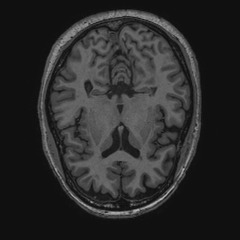
\includegraphics[width=.99\linewidth]{./images/t1.png}
 \end{minipage}
  \begin{minipage}{.32\textwidth}
 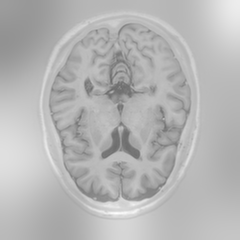
\includegraphics[width=.99\linewidth]{./images/t1-ir.png}
  \end{minipage}
  \begin{minipage}{.32\textwidth}
 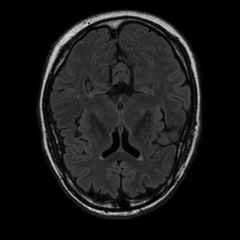
\includegraphics[width=.99\linewidth]{./images/t2-flair.png}
  \end{minipage}
  
   \begin{minipage}{.32\textwidth}
 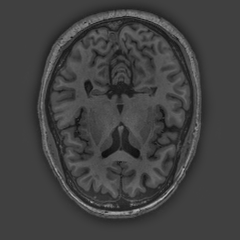
\includegraphics[width=.99\linewidth]{./images/t1-gs.png}
 \end{minipage}
  \begin{minipage}{.32\textwidth}
 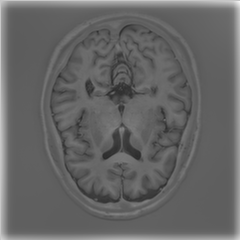
\includegraphics[width=.99\linewidth]{./images/t1-ir-gs.png}
  \end{minipage}
  \begin{minipage}{.32\textwidth}
 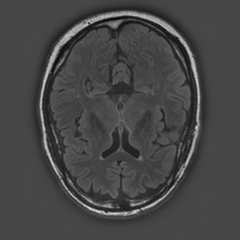
\includegraphics[width=.99\linewidth]{./images/t2-flair-gs.png}
  \end{minipage}
  \caption{Slice 19 of the 5th training sample. \emph{Top row (left to right):} T1, T1\_IR and T2\_FLAIR. \emph{Bottom row:} respective highpass filtered versions.}
  \label{data}
\end{figure}

\end{document}
